\section{Introduction}
Nowadays, there are countless bytes of data generated every second. In order to make best use of these data, we build datacenters (DC) which are distributed across the world and process data by running data analytic jobs in the slots of DCs. Thus, we need to design a strategy to arrange these jobs to minimize the overall run time so that the throughput of the whole system can be optimized. However, to solve this problem, we will encounter several challenges as below.
\begin{enumerate}
    \item Each job is composed of several computation stages among which there are precedence constraints, which can be described in a directed acyclic graph (DAG). As a result, the tasks in different stages can not be arranged simultaneously. Also, the arrangement of the previous step may influence the available slots and arrangement of the next stage.
    \item The data on which one job depends are geographically dispersed and the bandwidth between two DCs is limited. In addition, the topology of the network is not necessarily fully connected, which means data should be transmitted between DCs.
    \item The number of slots in each DC is limited, which means tasks may have to wait after it is ready for running.
    \item In addition to minimize the average completion time of all jobs, we have to maintain \emph{max-min fairness}. However, these two optimization objectives are in contradictory to some extend.
\end{enumerate}

To address these challenges, we designed a multi-module scheduling model (Fig. \ref{Fig-Flowchart}), which consists of a DAG scheduler, a dependency-free task scheduler and a simulator to emulate a real production environment with multiple DCs. Our overall strategy is stage-wide greedy, i.e. we keep the average completion time of each stage as short as possible to make the total completion time as short as possible. Here, we use the DAG scheduler to get the tasks for each stage which are dependency-free. To achieve a fair scheduling algorithm, Chen \emph{et al.} \cite{LP-paper} have proposed a linear-programming-based approach. We extract the core idea from it and give a network-flow-based approach to achieve similar results.
\begin{figure}
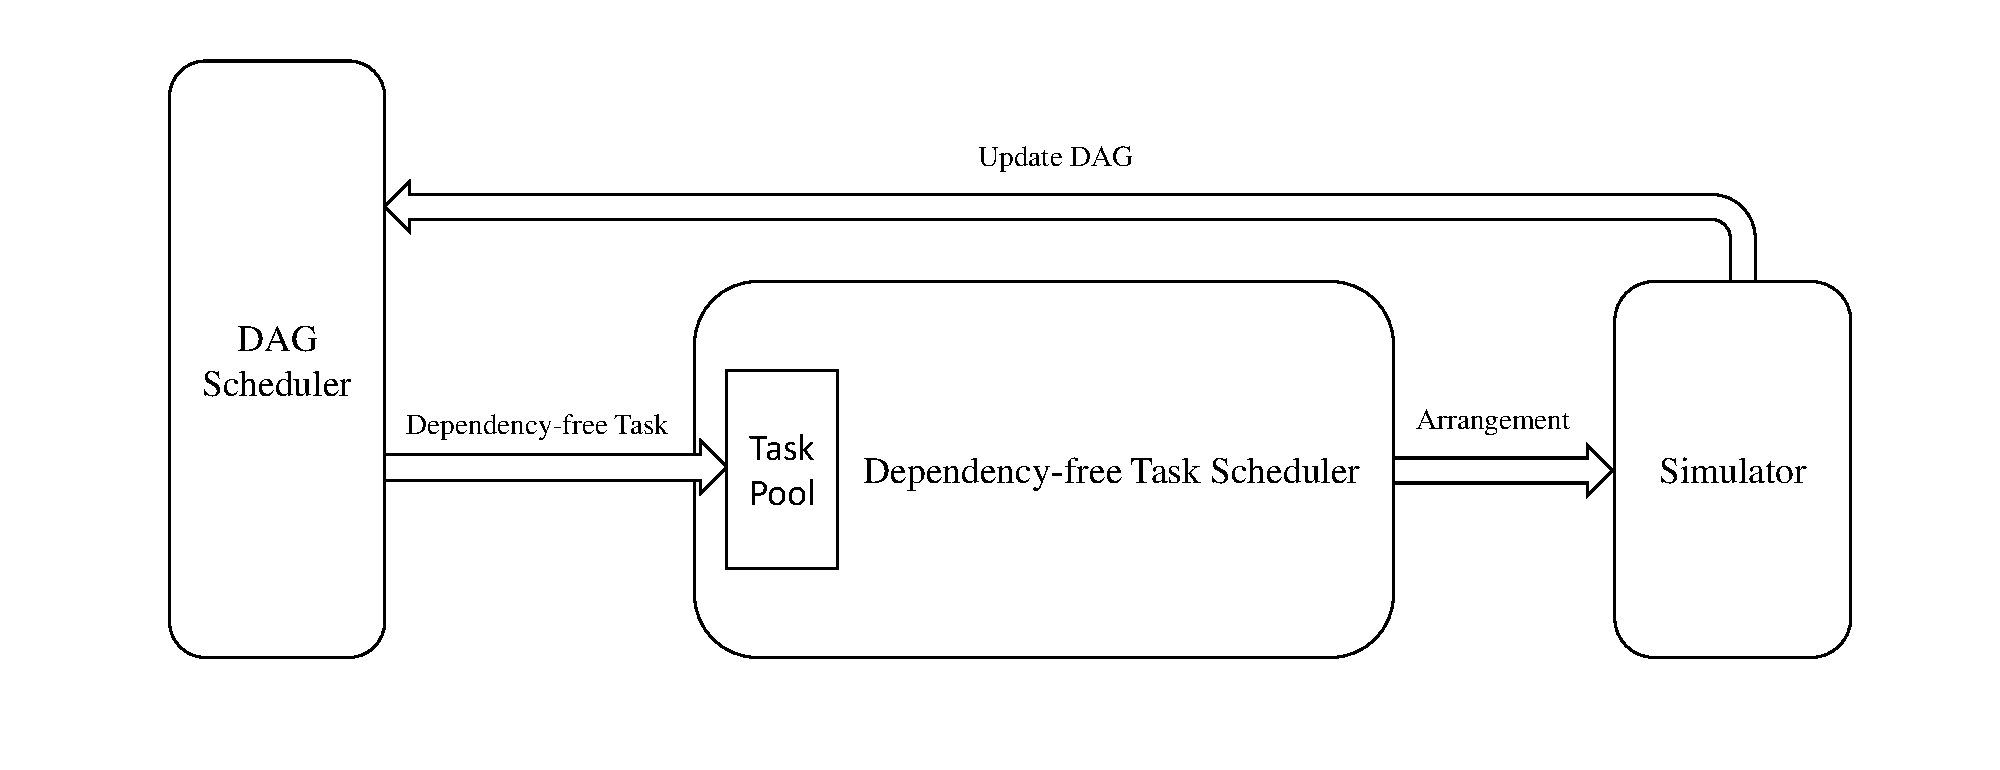
\includegraphics[width=0.8\textwidth]{figure/Fig-FlowChart.pdf}
\centering
\caption{Flowchart of the Model} \label{Fig-Flowchart}
\end{figure}
% \subsection{A Subsection Sample}
Please note that the first paragraph of a section or subsection is
not indented. The first paragraph that follows a table, figure,
equation etc. does not need an indent, either.

Subsequent paragraphs, however, are indented.

\subsubsection{Sample Heading (Third Level)} Only two levels of
headings should be numbered. Lower level headings remain unnumbered;
they are formatted as run-in headings.

\paragraph{Sample Heading (Fourth Level)}
The contribution should contain no more than four levels of
headings. Table~\ref{tab1} gives a summary of all heading levels.

\begin{table}
\caption{Table captions should be placed above the
tables.}\label{tab1}
\centering
\begin{tabular}{|l|l|l|}
\hline
Heading level &  Example & Font size and style\\
\hline
Title (centered) &  {\Large\bfseries Lecture Notes} & 14 point, bold\\
1st-level heading &  {\large\bfseries 1 Introduction} & 12 point, bold\\
2nd-level heading & {\bfseries 2.1 Printing Area} & 10 point, bold\\
3rd-level heading & {\bfseries Run-in Heading in Bold.} Text follows & 10 point, bold\\
4th-level heading & {\itshape Lowest Level Heading.} Text follows & 10 point, italic\\
\hline
\end{tabular}
\end{table}

\noindent Displayed equations are centered and set on a separate
line.
\begin{equation}
x + y = z
\end{equation}
Please try to avoid rasterized images for line-art diagrams and
schemas. Whenever possible, use vector graphics instead (see
Fig.~\ref{fig1}).

\begin{figure}
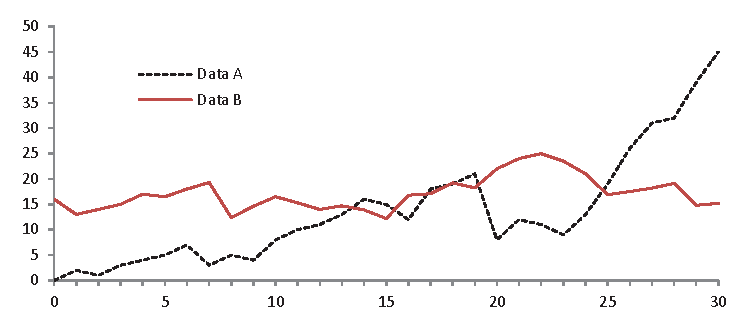
\includegraphics[width=0.6\textwidth]{figure/fig1.eps}
\centering
\caption{A figure caption is always placed below the illustration.
Please note that short captions are centered, while long ones are
justified by the macro package automatically.} \label{fig1}
\end{figure}

\begin{theorem}
This is a sample theorem. The run-in heading is set in bold, while
the following text appears in italics. Definitions, lemmas,
propositions, and corollaries are styled the same way.
\end{theorem}
%
% the environments 'definition', 'lemma', 'proposition', 'corollary',
% 'remark', and 'example' are defined in the LLNCS documentclass as well.
%
\begin{proof}
Proofs, examples, and remarks have the initial word in italics,
while the following text appears in normal font.
\end{proof}
For citations of references, we prefer the use of square brackets
and consecutive numbers. Citations using labels or the author/year
convention are also acceptable. The following bibliography provides
a sample reference list with entries for journal
articles~\cite{ref_article1}, an LNCS chapter~\cite{ref_lncs1}, a
book~\cite{ref_book1}, proceedings without editors~\cite{ref_proc1},
and a homepage~\cite{ref_url1}. Multiple citations are grouped
\cite{ref_article1,ref_lncs1,ref_book1},
\cite{ref_article1,ref_book1,ref_proc1,ref_url1}.